\documentclass{article}
\usepackage{amsmath}
\usepackage{tikz}

\usetikzlibrary{math}

\begin{document}

    \begin{center}
        \Huge
        Cochleoid curve
        \bigskip
        \normalsize
        
        Polar equation:
        \[r\left(\theta\right)=\dfrac{a\sin \theta}{\theta}\]
        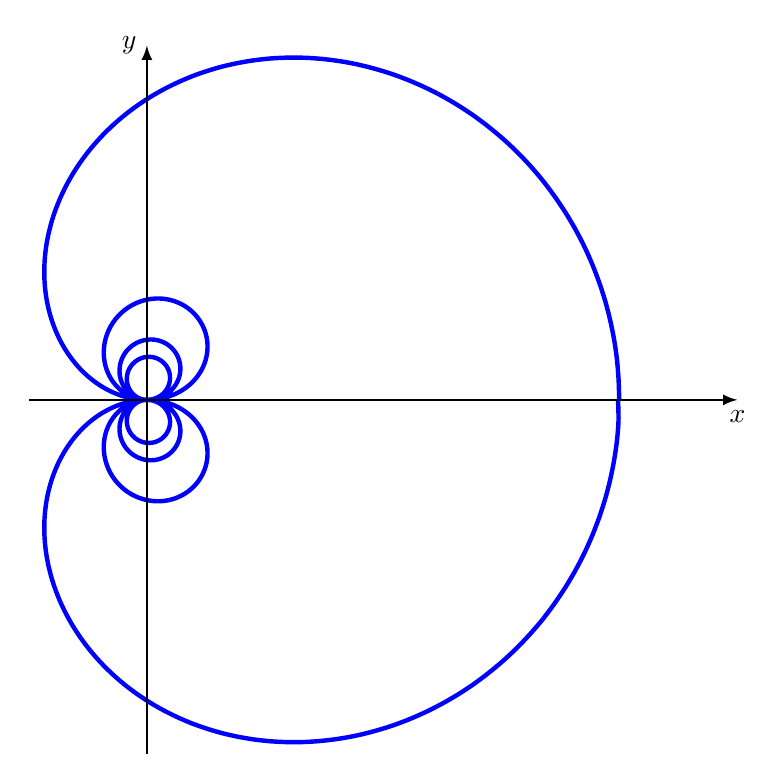
\begin{tikzpicture}[scale=1.5]
            \draw[color=blue, ultra thick, domain=0.1:360*2,smooth,variable=\t, samples=300] 
                plot ({\t}:{(4*sin(\t))/(\t*pi/180)});
            \draw[color=blue, ultra thick, domain=-360*2:-0.1,smooth,variable=\t, samples=300] 
                plot ({\t}:{(4*sin(\t))/(\t*pi/180)});
    
            \draw[thick, ->, >=latex] (-1,0) -- (5,0) node[below]{\(x\)};
            \draw[thick, ->, >=latex] (0,-3) -- (0,3) node[left]{\(y\)};
        \end{tikzpicture}    
    \end{center}

\end{document}
